\documentclass[12pt]{article}
\usepackage[a4paper, total={7in, 9.5in}]{geometry}
\usepackage[english]{babel}
\usepackage{indentfirst}
\usepackage{fancyhdr}
\usepackage{setspace}
\usepackage{graphicx}
\usepackage{hyperref}
\usepackage{epsfig}
\usepackage{paralist}
\usepackage{lastpage}
% \usepackage[scaled]{helvet}
% \renewcommand\familydefault{\sfdefault}
\usepackage[T1]{fontenc}
\usepackage{url}
\usepackage{pgfplots}
\usepackage{tocbibind}
\usepackage{amsmath}
\usepackage{enumitem}
\usepackage{algorithm}
\usepackage[toc,page]{appendix}

\pgfplotsset{compat=1.17}

\usepackage{xpatch}
\xpretocmd{\part}{\setcounter{section}{0}}{}{}

\pagestyle{fancy}
\fancyhf{}

\hypersetup{
  colorlinks=true,
  citecolor=blue,
  filecolor=black,
  linkcolor=blue,
  urlcolor=blue
}

\setlength{\parskip}{6pt}

\renewcommand{\headrulewidth}{0.3mm} % Top line width
\renewcommand{\footrulewidth}{0mm} % Bottom line width

\singlespacing

 \lhead{\hspace*{0mm}\raisebox{3mm}{
   \epsfig{file=~/Academia/TEX-Latex/logo/Aalto_en_1.pdf, height=11mm}}
 }

\chead{\hspace*{50mm}\raisebox{7mm}{\hspace*{60mm}\small\begin{tabular}{r}
      \textbf{Programing Studio 2}\\CS-C2120\\\today\\
\end{tabular}}}

%Footer
\lfoot{}
\cfoot{}
\rfoot{\thepage}

\newcommand{\argmax}{\operatorname*{argmax}}
\newcommand{\argmin}{\operatorname*{argmin}}

\begin{document}

\begin{titlepage}
    \thispagestyle{fancy}
    \begin{center}
        \vspace*{1cm}
            
        \huge
        \textbf{Documentation}
            
        \vspace{0.5cm}
        \Large
        Balancer\\

        \normalsize
        \vspace{0.5cm}
        Final Project for CS-C2120
            
        \vspace{1.5cm}
            
        \textbf{Hau Phan}

        \normalsize
        886690
            
        \vfill

            
        Bachelor Degree in Science\\
        Data Science Program\\
        Years of study: 2020-2023
            
        \vspace{0.8cm}
            
        \normalsize
        Department of Computer Science\\
        Aalto University\\
        Finland, \today
    \end{center}
\end{titlepage}
\newpage

\tableofcontents
\addtocontents{toc}{\protect\hypertarget{toc}{}}
\newpage

\section{General Description}
A strategy game where players tries to place weights on a set of scales while
keeping the scales balanced. The "riskier" the weight, the more score it yields.
Player with the most score win the round. The game spans over multiple rounds
and the winner is determined by the number of rounds won.
\subsection{Concepts}
\subsubsection{Weight}
A simple weight that has some \textit{mass}. All weights have the same mass. The
farther the weight from the scale center, the more \textit{score} it yields.
Weights can be stacked to form a \textit{stack} of weights.
\subsubsection{Scale}
A scale is a supported \textit{board} on which you can place other scales and
weights. Each board has two \textit{arms}: the left arm and the right arm.
\begin{verbatim}

                               A
                           A   A       A     A
                          <1=A=1>   <3=2=1=?=1=2=3>
                             b             a
                             *           A *
                        <5=4=3=2=1=?=1=2=3=4=5>
                                   a
                                   *
               XXXXXXXXXXXXXXXXXXXXXXXXXXXXXXXXXXXXXXXXXXXXX
\end{verbatim}

The farther the weight from the center of the board, the more torque it applies
to the scale's arm. The \textit{imbalance} measures the difference between the
torques. Note that a small imbalance is permissible. The maximum allowed
magnitude of imbalance is the same as if a weight was placed at the end of the
scale before the other weights were set. That is, for a \textit{balanced} scale,
the total imbalance $\geq$ the \textit{radius} of the scale. (See examples
below).  Once a scale is \textit{flipped}, it will be removed along with all its
weights.

\newpage
\textbf{Example 1}
\begin{verbatim}

                   A
         A         A
        <3=2=1=A=1=2=3>
               a
               *
    XXXXXXXXXXXXXXXXXXXXXXXX
\end{verbatim}

If a weight is at a distance of 3 from the center, it pushes that
arm down with the force of three weights. If the other side has two weights at
a distance of 2, they push that side down with a force of four weights. (2 * 2
= 4). The imbalance is 3 - 4 = -1. The absolute value of the imbalance is less
than the radius of the scale, 3, thus, the scale is balanced.

\textbf{Example 2}

If the left arm of the previous example did not have a weight, the scale would
have been \textit{unbalanced} (flipped) since the imbalance would have been 4,
exceeding the radius of the scale. In this situation, the scale is flipped and
all the weights is lost.  

You can also place other scales on the scale. The scale placed on the second
scale applies a force equal to the sum of the weights and scales on it.

\textbf{Example 3}

\begin{verbatim}

             A
         A   A       A     A
        <1=A=1>   <3=2=1=?=1=2=3>
           b             b
           *           A *
      <5=4=3=2=1=?=1=2=3=4=5>
                 a
                 *
                 *
    XXXXXXXXXXXXXXXXXXXXXXXXXXXXXXXX
\end{verbatim}

Scale $b$ is balanced, the right-side weighs 2 * 1 and the left one 1 * 1 which
does not exceed the radius of the scale. The scale B itself weighs three
weights.

Scale $c$ is balanced since the left side weighs 1 * 2 = 2 and the right side 1
* 1 = 1. The difference of these is 1, which does not exceed the radius of the
balance. Scale $c$ weighs 2 weights!

Scale $a$ is also balanced. On the left side there is a scale $b$ at a distance
of 3, 3 * 3 = 9. On the right there is scale $c$ at a distance of 4, 2 * 4 = 8,
and a weight at a distance 3. All together there is a weight of 11 weights on
the right side. The difference is 11 - 9 = 2, which is smaller than the radius
of scale $a$, so the scale is balanced.

\subsubsection{Players}
There are two type of players: \textbf{human} and \textbf{bot}. Multiple players
(recommended 2-3) can play the game at any one moment.
\subsubsection{Capture and ownership}
\label{sec:cap}

Both the \textbf{weights} and \textbf{scales} during each round are either
\textbf{player-owned} or \textbf{wild} i.e owned by no one. The wild weights and
scales are placed randomly at the beginning of each round and can be
\textit{captured} by players. Players can also capture each other weights and
scales. Captured scales give addition "buffs" for the owner's weights and
captured weights give points. Initially, when the weight is placed by a player,
it belongs to that player.


Weights can be \textbf{stacked}. One can capture all the weights underneath by
placing his/her weights on top. To capture a scale, one must have \textbf{at
least} $r$ more weights than the player with the 2nd most weights on the scale,
where $r$ is the radius of the scale. (See examples below)

Owner of a scale will have the following benefits:
\begin{itemize}
  \item His/her weights on the scale become \textit{resilient}: they can not be
    captured, even when other players place their weights on top. The moment the
    scales' owner changes, all weights that should be captured will be updated
    according to the rules.
  \item Each of his/her weight on the scale will yield twice the amount of
    points.
\end{itemize}

\textbf{Example:}
\begin{verbatim}
                   A
             A B   A C
            <2=1=A=1=2>
                 a     
                 *     
                 *    
       XXXXXXXXXXXXXXXXXXXXX
\end{verbatim}

Here the scale is captured by player A, since there are 3 A weights and only 1 B
and C weight. The difference is $3 - 1 = 2 \geq 2$ the radius of the scale. The
letter A in the middle indicates the owner of the scale.


\subsection{Rules and Gameplay} 
\subsubsection{Gameplay}
\begin{itemize}
  \item There is a predefined number of round per game. (Usually 5 for 2-3
    players)
  \item Each round will have a fixed number of weights that players can draw
    from and place onto the scales. (Usually 10-15 weights per round)
  \item At the beginning of each round, one scale and 5 wild weights will be
    randomly placed with some predefined probability.
  \item The round starts and the players place their weights one at a time on
    the scales. 
  \item The round ends when there is no weight left. The scores are then
    calculated and the player with the highest score win the round.
  \item The next round then starts and \textbf{continues} from the last round.
  \item The player who won the most round wins the game.
\end{itemize}
\subsubsection{Scoring}

\textbf{Example:} 
\begin{verbatim}

            A
      A B   A
     <2=1=A=1=2>
          b          
          *         C B
          *   ?     C B
         <3=2=1=?=1=2=3>
                a
                *
                *
    XXXXXXXXXXXXXXXXXXXXXXXXXXXXXX
    Status: equalibrium 

    a: scale b: (2 * 1 + 1 * 2) * 2 = 8 points 
       scale a: 3 * 8 = 24 points
       -------------------------------
       total: 24 points

    b: scale b: 1 * 1 = 1 points
       scale a: 3 * 1 + 3 * 2 = 9 points
       -------------------------------
       total: 9 points

    c: scale a: 2 * 2 = 4 points
       -------------------------------
       total: 4 points
\end{verbatim}

Here '$?$' represents wild weights and uncaptured scales. 

The scale with code 'b' is capture by the player 'A' so its points is multiplied
by 2.

\subsection{Difficulty level}
Completed level of difficulty: Intermediate/Difficult.

The project succeed in meeting all the requirement of Easy and Intermediate
criterions. Both a console-based and graphical user interface was implemented.
To meet the Difficult level's requirements, an intelligent computer opponents
was implemented along with additional game mechanics such as capturing scales,
weights and random computer-generated scales, undo/redo,\dots. The project also
aims at a creating a fully functional game: splash art, animations and tile
textures were also added to improve the game's visual.

\section{User interface}

\subsection{Graphical}

\subsubsection{Game loop}

When the user opens the game, a splash screen is shown with an animated logo and
background. The user can click on the top left of the menu bar to start a new
game, load a saved game or quit.

If the user chooses to start a game, the game will then switch to the game scene
where player can interact with the game. 

The game screen is shown on the left side of the window. Player can click
directly on the scale to place the weight, dragging to pan and scrolling to zoom
in and out.

The game information is shown on the right side of the window. This includes the
score and the number of rounds won by each player, the current round number and
how many weights left in the pool, \dots. There are also undo and redo buttons
to undo previous moves, and buttons to add additional scales and weights if
needed.

At the end of the round, a pop-up will be shown and announce the round's winner.
The game then continues to the next round, placing 5 weights and a scale at a
random position. If it is the final ground, a pop-up will announce the game's
winner instead.

\begin{figure}
  \centering
  \caption{The splash screen}
  \includegraphics[width=\textwidth]{graphic1.png}
  \label{fig:gra1}
\end{figure}
\begin{figure}
  \centering
  \caption{The game screen}
  \includegraphics[width=\textwidth]{graphic2.png}
  \label{fig:gra2}
\end{figure}
\subsubsection{Actions}

Player can choose to start a new game by clicking "File" > "New" or go back to
the menu with "File" > "Back to Menu".

At any moment, the user can choose to save the game by clicking "File" > "Save",
exit the game completely with "File" > "Exit" or go back to the splash screen by
choosing "File" > "Back to Menu"

\subsubsection{Settings/Options}

New players can be added by clicking the "Edit" > "Add Human" and "Edit" > "Add
Bot". Undoing and redoing moves can also be done in the "Edit" menu.

The rules and additional informations on the game can be accessed via the "Help"
menu in the menu bar.

The source code is also available by clicking the "Help" > "Github" and "Help" >
"Gitlab", which will open the repository using the default browser.

\subsection{Console-based}
The program can be run on the command line with no arguments to start a new game
or path to the save file to resume. A sample console output are shown below:

\begin{verbatim}
============ ROUND  1 ============
_________________________________________
| Ben   (B, 0) :    56 points (human)   |
| Ken   (K, 0) :   248 points (  bot)   |
| Jaiden (J, 0) :    63 points (  bot)  |
|_______________________________________|




       <5=4=3=2=1=?=1=2=3=4=5>
                  g
                  *
            J K   *   K K
           <4=3=2=1=?=1=2=3=4>
                    e
              ?     *
              B J   *       ?
             <2=1=?=1=2>   <1=?=1>
                  d           f
      K           *           *
      K           *           *
      K K         *           *
      K K         *         ? *     B
      K K     J ? *         K *   ? B
     <3=2=1=K=1=2=3>       <2=1=?=1=2>
            c                   b
            *       ? J   B     *
    ?   ?   *   B   B J   B J J *
   <7=6=5=4=3=2=1=?=1=2=3=4=5=6=7>
                  a
                  *
XXXXXXXXXXXXXXXXXX*XXXXXXXXXXXXXXXXXXXXXX
>>>>>>>>> BEN   TURN <<<<<<<<<
Which scale ? (d,b,g,e,f,c,a): a
Position ? [-7,7]: 1
\end{verbatim}

\subsubsection{New Game}

When a new game starts the game will prompt the user to enter basic information
about the players. The first round then starts and each player will in turn be
prompted for information on where his/her weight should be placed. The
scoreboard and the state of the game will also be shown to the players to help
them making their decisions.

When a round finished, the winner of the round will be announced. At the end of
the game, the final winner will be announced instead. The announcements are
simple outputs to the consoles.

\subsubsection{Load Game}

When the save file is loaded successfully, the game will continue from the state
when it is saved. If an error occurred, the line causing the failure will be
printed.

\section{Program Structure}

\begin{figure}
  \centering
  \caption{The balancer package structure}
  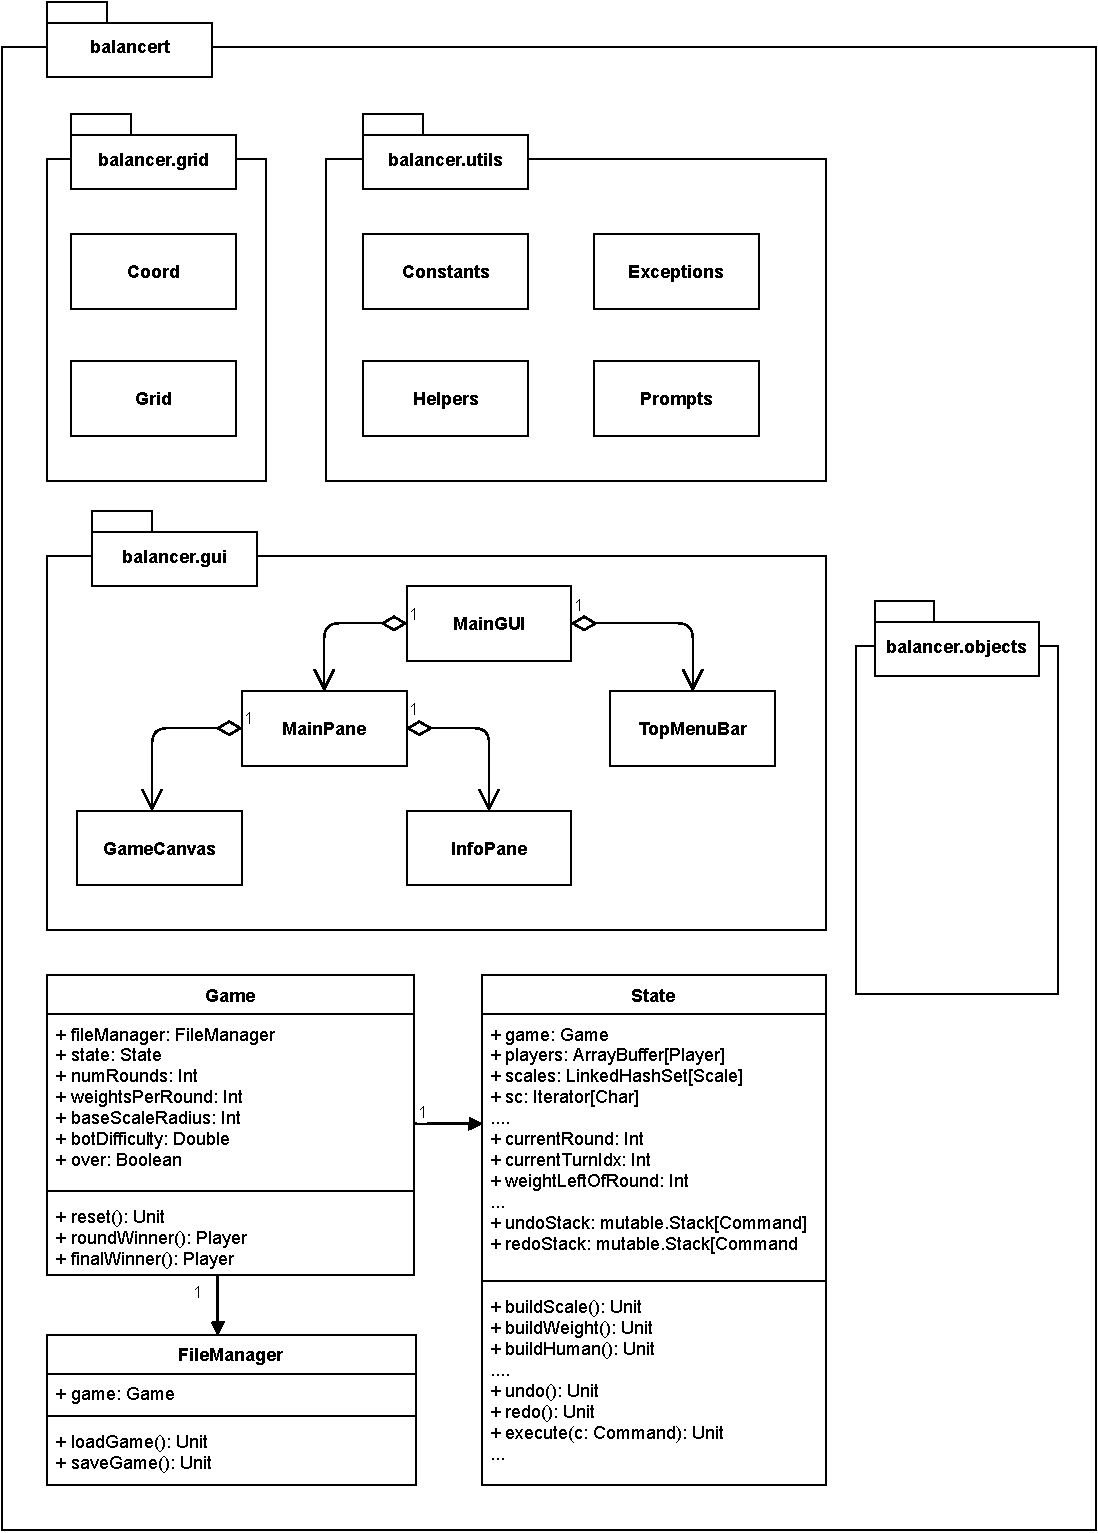
\includegraphics[width=\textwidth]{UML1.pdf}
  \label{fig:uml1}
  \caption{balancer.objects UML}
  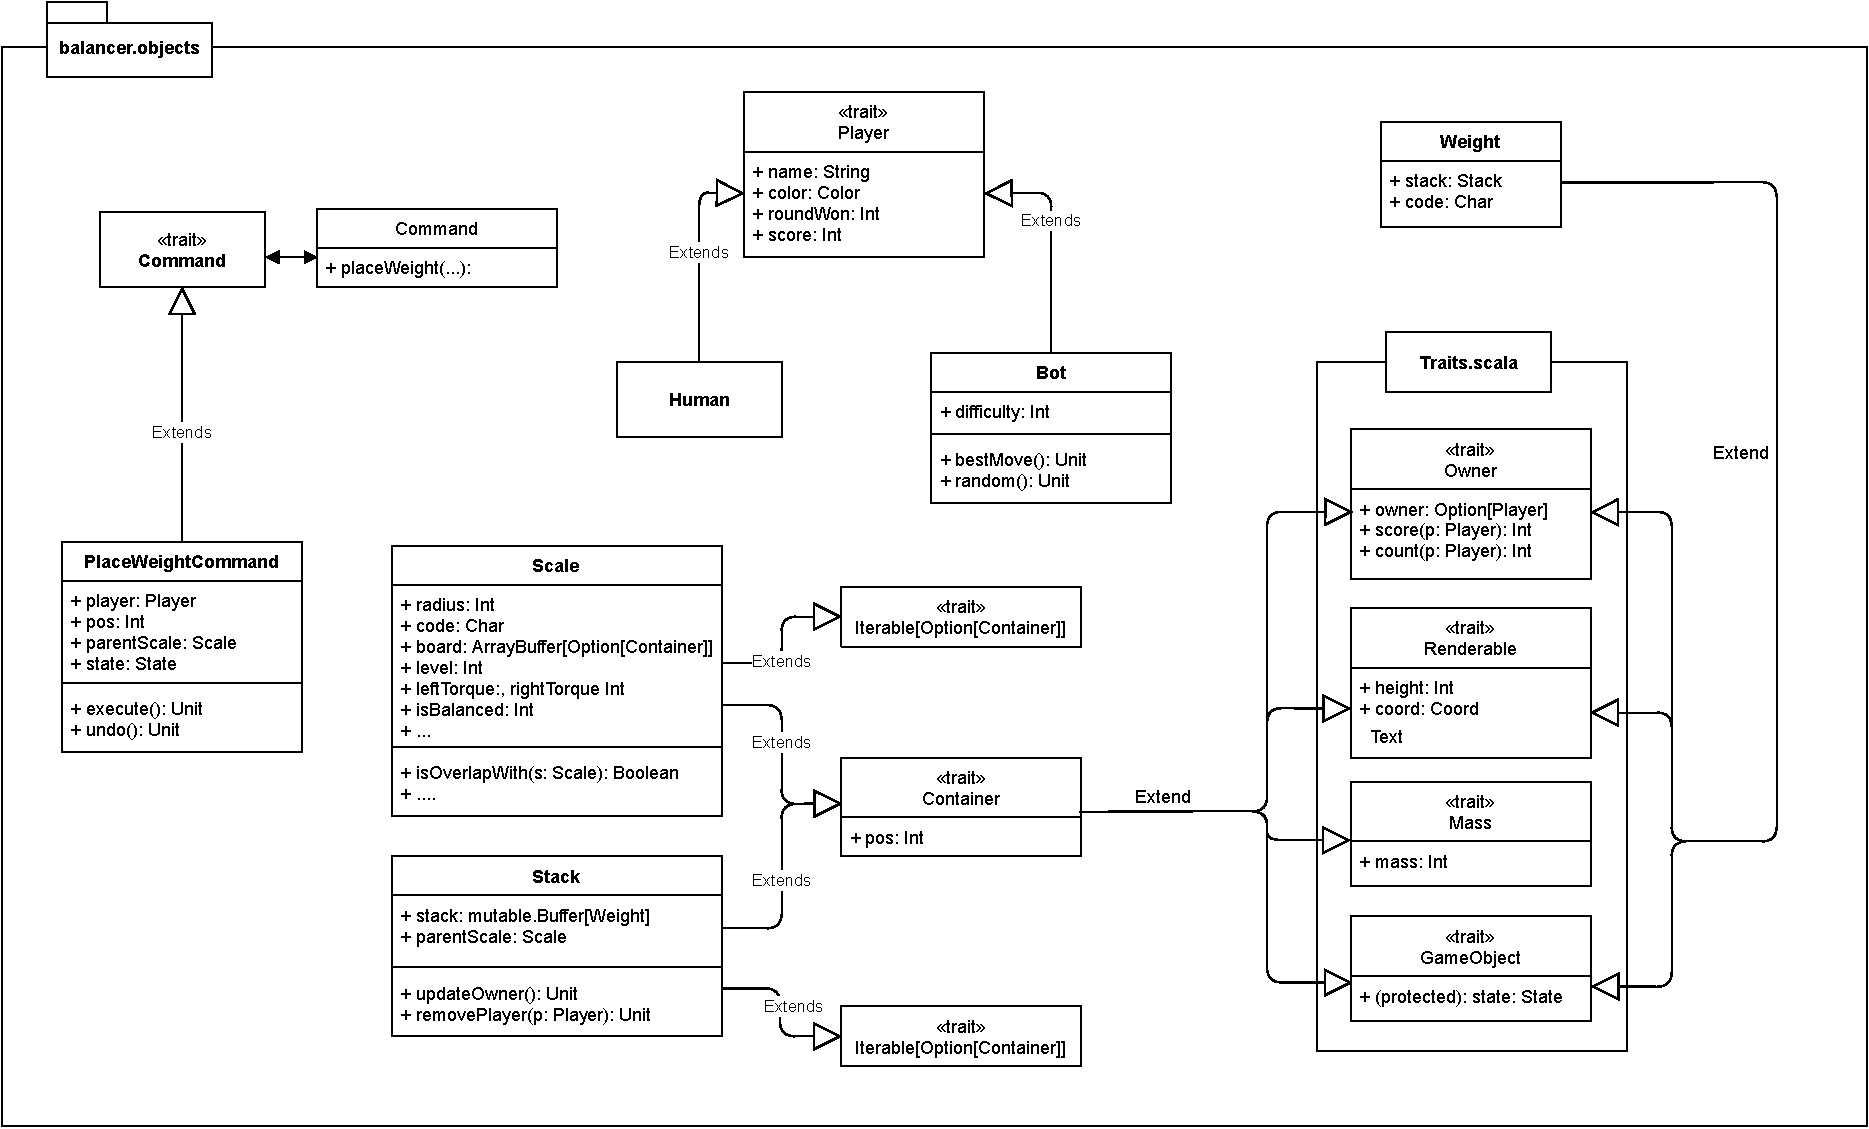
\includegraphics[width=\textwidth]{UML2.pdf}
  \label{fig:uml2}
\end{figure}

The program is split into packages, categorized according to their
characteristics and roles in the program. The top most package is named
\textit{balancer}, containing the classes \textbf{Game}, \textbf{FileManager}
and \textbf{State}. \textbf{Game} stores basic default settings of the game such
as the number of weights per round and the default difficulty of the bots. It
also acts as a mounting point for \textbf{State}, which is different for each
game and thus, changes whenever the users save or load.  \textbf{FileManager}
handles all operations regarding saving and loading \textbf{State}.
\textbf{State} models the game's state, which consists of any relevant
information that change during the game and methods that modify them.
\textbf{State} thus are unique for each game. The subpackages of
\textit{balancer} are:

\begin{itemize}

  \item \textit{balancer.grid:} containing the class \textbf{Grid} and
    \textbf{Coord}. \textbf{Grid} models a grid of character, an abstract
    representation of the game state. Each character either represent a weight
    belonging to a player, a part of the scale's board or an empty space. In
    other terms, \textbf{Grid} are just a collection of tiles used to display
    the game. \textbf{Coord} models a simple 2D coordinate or point, with basic
    arithmetic operations such as adding and subtracting.

  \item \textit{balancer.utils:} containing the objects \textbf{Constants, Helpers,
    Prompts} and \textbf{Exceptions}. \textbf{Constants} and \textbf{Helpers}
    are quite self-explanatory, they're comprised of different constants and
    helper functions. \textbf{Prompts} stores wrappers of the default ScalaFX's
    \textit{Alert} class. They range from informing the users, prompting for
    user inputs and opening the file-chooser dialog.

  \item \textit{balancer.gui:} containing wrappers of ScalaFX's components and
    \textbf{MainGUI}, which is the entry point of the application.
    \textbf{MainPane} is a wrapper class of ScalaFX's SplitPane, modeling the
    main area of the game. \textbf{TopMenuBar} extends the scalafx's MenuBar,
    modeling the app's menu bar, while \textbf{GameCanvas} extends the default
    scalafx's ScrollPane, allowing for panning and zooming. A canvas is also
    attached to display the game's grid. \textbf{InfoPane} is the left pane in
    charge of display other relevant stats/information about the game, such as
    the score of each player and the number of weights left in the round.
    Modifying the game's state and the players's indicator color can also be
    done from \textbf{InfoPane} 

  \item \textit{balacner.objects:} containing objects that model different
    aspect of the game's mechanics and gameplay. The relationships between them
    are shown in Figure \ref{fig:uml2}. \textbf{Command} models a command or a
    move from a player. For now, there is only one command: the place weight
    command. \textbf{Scale} and \textbf{Stack} models the in-game scale and
    stack of weights. \textbf{Traits.scala} stores shared traits between
    \textbf{Scale}, \textbf{Stack} and \textbf{Weight}.  \textbf{Stack} and
    \textbf{Scale} also implements the methods of Scala's \textbf{Iterable},
    allowing it to be looped over and its content accessed with index, similar
    to scala's \textbf{Seq}.  \textbf{Player} models a generic player, with a
    unique name, color and basic stats such as the number of round won and
    score.  \textbf{Human} and \textbf{Bot} extend from \textbf{Player},
    modeling a human player and a bot player respectively.

\end{itemize}

\section{Algorithms}
\subsection{Attributes}
Due to the recursive nature of the game (scale on scale on scale), most methods
and attributes are either call other recursive methods or recursively defined:
\begin{itemize}
  \item scale's \textit{mass} = the sum of its stack's \textit{mass} and its
    child scales's \textit{mass} 

  \item stack's \textit{mass} = the sum of its weight's \textit{mass}

  \item scale's \textit{level} = its parent scale's \textit{level}  + 1 (0 if at
    the bottom)

  \item scale's \textit{imbalance}: 
    \begin{align*}
      \text{Imbalance} = \sum_{i=-r}^{r}i\;m_i
    \end{align*}
    where $r$ is the radius of the scale, $m_i$ is the mass of the object at
    distance $|i|$ from the center. Negative value of $i$ indicates the object
    is on the left arm of the scale.

  \item \textit{score}: player $p$'s \textit{score} on an object $o$ is a
    piecewise function conditioned on $o$ and $p$:
    \begin{equation*}
      s(o,p) = \begin{cases}
        s(o, p) = \sum_{i=-r}^{r} |i|\;s(o_i, p) , &\text{ if $o$ is a scale}\\
        s(o, p) = \sum_{w\in S} s(w, p) , &\text{ if $o$ is a stack, with
        weights $S$}\\
        s(o, p) = 1 &\text{ if $o$ is a weight owned by $p$}\\
        s(o, p) = 0 &\text{ if $o$ is a weight not owned by $p$}
      \end{cases}
    \end{equation*}
    where $o_i$ is the object at distance $|i|$ from the center the scale.
    Negative $i$ indicates the object is on the left arm.

  \item \dots
\end{itemize}
\subsection{Intelligent bot}
\subsubsection{Description}
\begin{itemize}
  \item \textbf{randomized:} The randomized bot simply searches for all moves
    and filters out moves that would tip a scale, then randomly picks a move.
  \item \textbf{semi-greedy:} The semi-greedy bot also searches for all moves
    and filters out moves that would tip a scale, but then picks the move that
    yields the most point for the bot instead.
  \item \textbf{mixed:} a random number generator is used to determine which
    algorithm to between the above twos.
\end{itemize}
The \textbf{randomized} bot can check if a move will result in any flipped scale
by "faking" the move: places the weight, recursively checks if any scale is
flipped then reverts/undo the move. Similarly, the \textbf{semi-greedy} bot can
implement a similar method and calculate the score before reverting back, thus
finding the move that yield the highest score.

Computing time is nearly instant for most game with human players, which should
be at most 10 scales per round. 

\subsubsection{Limitations}
Since the bot will never tip a scale, human players can exploit this
characteristic of the bot and flip a scale deliberately at key moments to come
out on top. A true greedy bot will also takes moves that will tip a scale into
consideration and choose weather to disrupt the human players or not.

\subsection{Randomized Generation}

\textbf{Avoiding collision when generating scale}: 
A simple brute force algorithm is implemented to place random scale without them
overlapping each other: finding all empty positions, randomly pick a position,
"fake" placing the scale and check if collide with any scale of the same level,
if it is, revert the placement.

\textbf{Weight generation:} 
A similar algorithm to the \textbf{random-bot} algorithm is used: Search for
all possible moves that wouldn't tip any scale if played, then randomly execute
one of those move to place a random weight on the scales.

\section{Data Structures}

\textbf{Grid} is implemented as a 2D \textbf{Array} of character (\textbf{Char})
due to it performance (constant access and insertion time). Since \textbf{Grid}
will be modified frequently (whenever there is a change in the game state),
quick access, insertion and initialization is crucial for performance. Since
most of the grid entries are empty, the grid is \textit{sparse}, and some
optimization can be done. Other data structures such as HashMap and R-Tree was
also considered to benefit from the sparseness of the matrix, such as reducing
memory usages. However, since the dimension of the grid is not too large ($<
10000$ entries), the memory saved/performance trade offs due to overheads might
not be desirable. Furthermore, for most modern computer, memory deficiency is
not a problem anyway. Implementing a grid as a 2D \textbf{Array} also help in
development due to its familiarity.

\textbf{State} also contains a collection of references to the scales, since
traversing the scale recursively might not be efficient for some operations. The
scales collection is implemented as Scala's mutable collection
\textbf{LinkedHashSet}, since we need a mutable collection of unique elements
with constant access time and good insertion time. However
\textbf{LinkedHashSet} is only used during development: since the elements are
ordered (scale inserted first will be accessed first), it is useful during
debugging and testing. During deployment, however, the normal \textbf{HashSet}
will be used instead to reduce overhead operations introduced by linking. The
program is designed to better handle large amount of scales.  However, as a
concession, it is known that the average number of scales might not exceed $10$
in most game with human players, thus \textbf{ArrayBuffer} might be a better
alternative. \textbf{State} will also stores a collection of \textbf{Player}
which be implemented as Scala's \textbf{ArrayBuffer}.

\textbf{Stack} is implemented as a \textbf{Buffer}, since it provides much of
the functionality of a stack and easy to work with.  The \textit{board} of
\textbf{Scale} will be modeled as a immutable \textbf{Array} since its length is
constant i.e the scale can not shrink or grow in length. Raw access speed and
low overhead is also one reason to choose the default \textbf{Array} over
\textbf{Buffer} for \textit{board}.


\section{File and Internet Access}

The state of the game is saved in a semi-human-readable format:

\begin{verbatim}
    BALANCER 1.0 SAVE FILE
    # Setting
    WeightPerRound: 15
    NumberOfRound: 5
    BotDifficulty: 0.5
    # Meta
    Human: Ben
    Bot: Ken,Jaiden
    Round: 1
    Turn: Ben
    # Scale
    _,0,7,a : -5,? | -1,B | 1,B | 2,J,J | 4,B,B | 5,J | 6,J
    a,7,2,b : -2,K | 2,B,B
    a,-3,3,c : -3,K,K,K,K,K | -2,K,K,K | 1,J | 2,?
    c,3,2,d : -2,B | -1,J
    d,1,4,e : -4,J | -3,K | 1,K | 2,K
    b,-1,1,f : -1,?
    END
\end{verbatim}

\begin{itemize}
  \item The first line of the file is of the form: 
    \begin{align*}
      \text{BALANCER (VERSION) SAVE FILE}
    \end{align*}
  \item The file is split into blocks. Each block of data has a header and a
    body. A header is identified by having "\#" prepended. The header marks the
    start of a block.
  \item Each row in the body contains information about the game and is of the
    form:
    \begin{align*}
      \text{IDENTIFIER : DATA}
    \end{align*}
    \item The IDENTIFIER and DATA is different for different blocks.  There are
      3 types of block: \textit{Setting, Meta} and \textit{Scale}.
  \item The \textit{Setting} block contains different configurations of the saved game.
  \item The \textit{Meta} block contains metadata of the saved game. 
  \item The \textit{Scale} block contains the position of each scales and weights when
    the game is saved. The IDENTIFIER is the scale's position and the DATA is
    the position of each weight on the scale:
  \item For example, this line in the \textit{Scale}  block:
    \begin{verbatim}
                        a,7,2,b : -2,K | 2,B,B
    \end{verbatim}
    from left to right indicates: the parent scale code ("a"), the position on
    the parent scale (on the right arm, distance 7 from the center) and the
    radius ($=2$) \item After the colon are the weights' position on the scale,
    it must be listed from left to right (thus the indices must be from smallest
    to biggest). 
    \begin{itemize}
      \item (-2,K) indicates on the left arm, distance 2 from the center, there
        is a weight belong to Ken (K).
      \item (2,B,B) indicates on the right arm, distance 2 from the center,
        there are 2 weights stacked on each other, both belong to Ben (B). The
        bottom weight is on the right.
    \end{itemize}
  \item The END keyword represents the end of the saved file. Any line after
    this keyword is not interpreted by the parser.
  \item \textit{Note: for the bottom most scale, the parent scale code is "\_",
    and the position is $0$. "?" indicates this is a wild weight or scale, i.e,
  with no owner. Any excess white space will be ignored by the parser.} 
\end{itemize}

\section{Testing}

The program is tested manually by typing onto the console (for text-only
version) or interacting with the graphical UI directly (in a graphical window).
The following aspect of the game was tested:
\begin{itemize}
  \item The weight is placed at the correct position according to the user mouse
    position.
  \item Panning and zooming work correctly.
  \item Information/status of the game such as the score, the round number and
    the number of weights are displayed correctly.
  \item \textbf{GameCanvas} accurately displays the current state of the game
    and update when a new weight is placed.
\end{itemize}

There are automated tools to system test graphical user interfaces. However,
running the game directly is the most straightforward one. Different save files
are created and purposely designed to test different aspects of the game,
specifically, accurate balance-checking of the scales, bot algorithms and random
weight, scale generation. 

Important "core" methods and attributes that are used frequently through out the
program are unit-tested. Example of these "core" methods are the
\textit{buildWeight()} and \textit{buildScale()} of \textbf{State}. They have
multiple test cases designed specifically to test there accuracy. Some tests
also aim to test how "solid" these methods are by simulating edge cases and
invalid inputs.

Beside "core" methods, algorithms are also tested frequently for accuracy, i.e
they do what they are supposed to do. The two algorithms that will be tested
intensively are the \textbf{semi-greedy} bot's algorithm and the rendering
algorithm for update the game's grid. 

Only some methods and algorithms passed the tests during their first
implementation. Most of them failed and reveal obscure bugs and faulty
logic in the code. The semi-greedy bot algorithm was most tested and also failed
the most. 

The loading and saving of game file is also tested intensively. There might
still be bugs in the implementation, however, since there are a lot of edge
cases and human-readable/modifiable save file has a lot of edge cases that
needed to be accounted for.

\section{Known bugs and missing features}

\subsection{Bugs and Temporary Fixes}

A possible area where bugs can occur is during the loading and saving of the
game. The custom parsing function \textit{loadGame()} was done rather "hacky",
which may contains obscure bugs that hard to identify. However, a general
try-catch safeguard was implemented to at least catch these errors and notify
the users about them.

Another possible bug that might occur is when there are players with similar
first letter name (e.g Jack and Jason, Mike and Mary\dots). Since the
\textit{weightCode} is the first letter of the its owner's name, their weights
will be represented by the same \textbf{Char} on the grid and considered as
belong to the same player. This is likely to cause weird behaviors in the game.
Thus, to prevent this, the game will throw an error and notify the player if
such naming collision happen.

There are also extreme game states that can be achieve if users want to
purposely breaking the game, such as adding infinite number of scales or
players. There is a max-depth limit for recursion in Java/Scala, thus, exceeding
this limit will cause the program to throw an error when executing/calculating
any recursive methods/attributes. The number of scales might also exceed the
limit for lowercase letter in ASCII ($z = 122$) and thus, assign weird
characters to newly added scales.  However, both of these problem can be fixed
by limiting the number of scales to $26$.

On the opposite side, the game might also have $0$ player or only consists of
bots. This is also likely to cause an error and thus, at least one human player
are required for the game to start.

\subsection{Missing Features}

\textit{Multiplayer supports:} The original plan includes implementing a basic
multiplayer version of the game using \textit{Play framework}'s Websocket.
However, overlapping schedules, heavy workload from other courses, it was not
realized.

\textit{Full Undo:} While undoing and redoing is not mentioned in the original
plan, they are additional features that I only manage to partially realized:
undoing is not fully implemented for scale. When a scale is flipped, no undoing
can be made to reinstate that scale.

\section{Best sides and Weaknesses}

\subsection{Best sides}
\begin{enumerate}

  \item The program is quite organized and can be easily expanded/build upon to
    accommodate additional features if needed. Each packages is separated
    according to its roles in the program: \textbf{Helpers} contains helper
    functions and \textbf{Constants} stores different constants that are used.
    GUI elements are modular, separated and explicitly named after their roles:
    \textbf{TopMenuBar}, \textbf{MainPane}, \textbf{GameCanvas}, \dots 

  \item Undoing and redoing were not planned in the original plan but are the
    results of refactoring to the class \textbf{Command}. While there are only
    one command implemented (\textbf{PlaceWeightCommand}), future commands such
    as \textbf{AddingPlayer}, \textbf{RemovePlayer}, \textbf{AddScale} ,
    \textbf{RemoveScale} \dots can easily be added using the same base class.

  \item Zooming and panning the \textbf{GameCanvas} was more complicated than
    expected, however a clean implementation was done and managed to work
    reliably.  The control is also quite intuitive: users can simply click,
    drag, pan similar to a normal touchscreen. The use of sprites and custom
    font also help making the game more visually appealing.  
\end{enumerate}

\subsection{Weaknesses}
\begin{enumerate}
  \item As mentioned above, the \textit{loadGame()} function to parse the game
    file is rather hacky and not really robust to changes.
  \item Updating of UI elements are done by calling a separate function and only
    called when needed (\textit{updateContent()} of \textbf{InfoPane} ).
    However, this is not easily scaled since a new line has to be added in the
    function every time a new UI element need to change dynamically. A better
    implementation would be using the default \textbf{Bindings} in
    scalafx.beans.binding, which would not only improve the performance of game
    but also the readability of the code.
  \item The algorithms are brute force algorithm and might not be
    efficient.  While they are easy to implement and understand, fake placing a
    weight might introduce additional complexity that could be avoided using a
    bottom-up approach (say filtering from all possible position the position
    that would flip the scale if place a weight there).
\end{enumerate}

\section{Deviations from the plan, realized process and schedule}

Most of the program was realized during the first two weeks (\textbf{22.2} -
7.3), which includes the core classes (\textbf{Weight, Scale, Stack, State, Game
\dots}), \textbf{FileManager}, all the algorithms (\textit{randomized} and
\textbf{semi-greedy}  and random placements), \textbf{MainText} (the console
version of the game) and most of the GUI components. At this point, the project
was mostly done and for a period of time, no progress was made due to
overlapping of other courses. The last two week (14.4 - \textbf{28.4}) was then
reserved for minor tweaking, testing, documenting and making the game more
visually appealing.

Here are the original plan and scheduling for comparison:
\begin{quote}
\begin{itemize}
  \item  The first two weeks (\textbf{22.2} - 7.3): build core classes.
    + bot algorithm 
  \item The week after (8.3 - 14.3): implement and test the save/load file
    functionality 
  \item  The next 2.5 weeks (15.3 - 31.3): build and test the UI for the game,
    on the console and graphically in a window
  \item  The next two weeks (1.4 -  14.4): system testing of
    the whole program, debugging, tuning, optimizing for performance and adding
    additional features where needed.
  \item The final two weeks (14.4 - \textbf{28.4}): documenting + "buffer zone"
\end{itemize}
\end{quote}

All the work for the first 5-6 weeks was done early during the first 2 weeks and
the final documentation/ testing was cramped in the last 2 weeks. In retrospect,
the difference between the planned schedule and reality are quite drastic and
unprecedented. The process deviated when I managed to implement the program
faster than expected. This was resulted from the abundance of free time I had at
the time. During the following weeks, since most of the project was done, I
focused on other courses and projects, which lead to a period of stagnation and
no progress was made. After the evaluation week was when I came back and work on
the project.

\section{Final Evaluation/ Self Assessment}

Overall the final result is quite satisfactory. Most of the main features of the
program are realized and working as expected. The program is also organized and
designed to be expandable, allowing for addition of new features and
improvements with out modifying large portions of the existing code. The program
while not at all stunning in term of graphic but at least is functional and not
visually decent. The bot's algorithms can be improve to be more efficient.
However, finding such a solution is a challenge in itself that I have not
managed to overcome.  Undoing and redoing are also features that are
surprisingly easy to implement given the program's class structures, which shows
the importance of planning in programming a large project.

However, there are also unwanted shortcomings. The save file, while is concise
and human-readable, are not robust and flexible. If users choose to create their
own saved file, it is likely that there will be typos or small mistakes,
producing obscure errors that are difficult to read and fix. Therefore, a more
popular structured file format such as JSON or XML should have been used in the
beginning instead. There are also some missing features that are mentioned
above, such as a fully functional undo that can undo flipped scale and
multiplayer support. Moreover, the update function to update UI components
should be removed and replaced by ScalaFX's bindings. The GUI portion of the
program can also be improved by using FXML for laying out the elements instead
of vanilla Scala with \textbf{Seq}. Using FXML can help with readability and
scalability, allowing for the development of complex UI structure if needed.

\nocite{nystrom2014game} 
\nocite{scalacollection} 
\nocite{scalafx}

\bibliographystyle{unsrt}
\bibliography{/home/phanth/Academia/TEX-Latex/bib.bib} 


\newpage

\begin{appendices}
\section{Illustrative Execution Examples}

\subsection{Console}
\begin{verbatim}

        Successfully load 'testfile.txt'
        Welcome to Balancer !!
        ============ ROUND  2 ============
        _________________________________________
        | Ben   (B, 0) :    48 points (human)  |
        | Ken   (K, 0) :    70 points (  bot)  |
        | Jaiden (J, 0) :    86 points (  bot)  |
        |_______________________________________|




                    K               B
                   <4=3=2=1=?=1=2=3=4>
                            e
                            *
                      ? ?   *
             <1=?=1> <2=1=?=1=2>   <1=?=1>
                g         d           f
              ? *         *           *
              K *         *           *   B
              K *         *         J *   J
              K *     ?   *         J *   J
             <3=2=1=?=1=2=3>       <2=1=J=1=2>
                    c                   b
                ?   * B     J           *
            K   ? ? * B B   J   ? ? ?   *
           <7=6=5=4=3=2=1=?=1=2=3=4=5=6=7>
                          a
                          *
        XXXXXXXXXXXXXXXXXX*XXXXXXXXXXXXXXXXXXXXXX
        >>>>>>>>> BEN   TURN <<<<<<<<<
        Which scale ? (d,b,e,f,c,a,g): a
        Position ? [-7,7]: 4
\end{verbatim}

\subsection{Graphical}
\begin{figure}
    \centering
    \caption{Game Screen loaded from file}
    \includegraphics[width=\textwidth]{graphic2.png}
    \label{fig:gra3}
\end{figure}

\begin{figure}
    \centering
    \caption{Game Screen after some round/ Changing the color}
    \includegraphics[width=\textwidth]{graphic3.png}
    \label{fig:gra3}
\end{figure}
\begin{figure}
    \centering
    \caption{Adding new Players}
    \includegraphics[width=\textwidth]{dialog1.png}
    \label{fig:dia1}
\end{figure}

\begin{figure}
    \centering
    \caption{Saving the game}
    \includegraphics[width=\textwidth]{dialog2.png}
    \label{fig:dia2}
\end{figure}

\end{appendices}
\end{document}
